\chapter{Mathematical Circuits Using Op.Amp.: Part I}


\section{Objectives}
\begin{itemize}
    \item 
    \item 
\end{itemize}

\section{Materials}
\begin{itemize}
    \item Breadboard
    \item DC power supply
    \item Digital Multi-Meter
    \item Function Generator
    \item \hyperref[LM741_1]{Op.Amp. (LM741)}
    \item Oscilloscope
    \item Resistors
\end{itemize}

\section{Introduction}
    \subsection{Operational Amplifier}
        \begin{itemize}
            \item \textbf{What is the Operational Amplifier}\par
                Operational Amplifier, normal written as Op.Amp., are fundamental components in electronics which is used in analog electronics. It is constructed using a combination of several MOSFETs.\par
                Op.Amp. is a high-gain voltage amplifier with a differential input (negative and positive inputs).\par
                Operational amplifiers are versatile components that can be utilized in a variety of applications, including signal amplification, waveform oscillation, and performing mathematical operations.
        \end{itemize}
    \subsection{Specification}
        \begin{itemize}
            \item \hyperref[LM741_1]{Op.Amp. (LM741)}
        \end{itemize}
        
    \subsection{Circuit Diagram}
    \begin{figure}[h]

        \begin{subfigure}[h]{0.47\textwidth}
        \begin{center}
            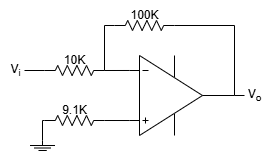
\includegraphics[width=1\linewidth]{Lab10/Lab10a.drawio.png}
            \caption{}
            \label{L10a}
        \end{center} 
        \end{subfigure}
    \hfill
    \vspace{0.2 cm}
        \begin{subfigure}[h]{0.47\textwidth}
        \begin{center}
            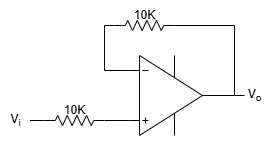
\includegraphics[width=1\linewidth]{Lab10/Lab10b.drawio.png}
            \caption{}
            \label{L10b}
        \end{center}
        \end{subfigure}
    \vfill
    
    \vspace{0.2 cm}
        \begin{subfigure}[h]{0.47\textwidth}
        \begin{center}
            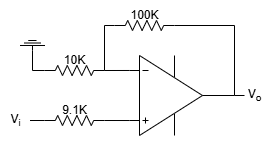
\includegraphics[width=1\linewidth]{Lab10/Lab10c.drawio.png} 
            \caption{}
            \label{L10c}
        \end{center}
        \end{subfigure}
    \hfill
        \begin{subfigure}[h]{0.47\textwidth}
        \begin{center}
            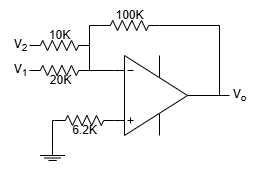
\includegraphics[width=1\linewidth]{Lab10/Lab10d.drawio.png}
            \caption{}
            \label{L10d}
        \end{center}
        \end{subfigure}

    \vspace{0.2 cm}
        \begin{subfigure}[h]{0.47\textwidth}
        \begin{center}
            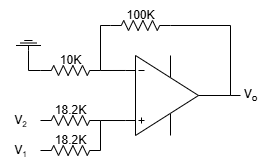
\includegraphics[width=1\linewidth]{Lab10/Lab10e.drawio.png}
            \caption{}
            \label{L10e}
        \end{center}
        \end{subfigure}
    \hfill
        \begin{subfigure}[h]{0.47\textwidth}
        \begin{center}
            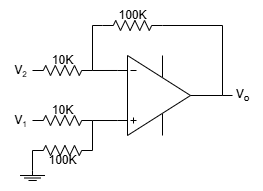
\includegraphics[width=1\linewidth]{Lab10/Lab10f.drawio.png}
            \caption{}
            \label{L10f}
        \end{center}
        \end{subfigure}
    \caption{Different fundamental Op.Amp. circuits}
    \label{l10fs}
    
    \end{figure}
    \FloatBarrier

\section{Detailed Procedures}
    \subsection{Analyzation}


    \subsection{Procedures}

    
\section{Discussion}


\section{Conclusion}